\documentclass[12pt,a4paper]{article}

\usepackage[utf8]{inputenc}
\usepackage[T1]{fontenc}
\usepackage[italian]{babel}
\usepackage{geometry}
\usepackage{graphicx}
\usepackage{booktabs}
\usepackage{float}
\usepackage{amsmath}
\usepackage{caption}
\usepackage{array}
\usepackage{tabularx}
\usepackage{hyperref}

\geometry{
    top=2.5cm,
    bottom=2.5cm,
    left=3.5cm,
    right=3.5cm
}

% Paragrafi allineati allo stesso margine sinistro
\setlength{\parindent}{0pt}
\title{Tumor hypoxia and survival in lung adenocarcinoma}

% Didascalia sopra le tabelle e sotto le figure
\captionsetup[table]{position=top}
\captionsetup[figure]{position=bottom}

\title{Ipossia tumorale e sopravvivenza nell'adenocarcinoma polmonare}
\author{Salvatore Megna}
\date{}

\begin{document}

\maketitle

\section{Introduction}

Lung adenocarcinoma is one of the main forms of non-small-cell lung cancer and is characterized by substantial clinical and biological heterogeneity among patients. This heterogeneity can translate into important differences in disease progression, treatment response and survival. To investigate these aspects, a dataset was assembled from the clinical and molecular data of the TCGA-LUAD PanCancer Atlas project (\textit{The Cancer Genome Atlas -- Lung Adenocarcinoma}), combining each patient's overall survival time, vital status, age at diagnosis, sex, pathological stage, histological subtype and molecular indicators associated with tumor hypoxia.

The specific objective of the analysis is to evaluate whether, and to what extent, patients' clinical and molecular characteristics are associated with overall survival. In particular, the study aims to assess whether biological markers related to tumor hypoxia provide additional prognostic information beyond the main clinical features, allowing the identification of profiles associated with different survival outcomes. Survival time is therefore analyzed using Kaplan--Meier curves, the log-rank test and the semiparametric Cox model. The main model assumptions are also assessed using appropriate diagnostic tools.

\section{Dataset}

\subsection{Dataset construction}

The data come from the TCGA-LUAD PanCancer Atlas study and were obtained through cBioPortal. The original clinical dataset contains 566 patients with lung adenocarcinoma and 40 variables. The dataset has a patient-level structure: each row represents one patient and no duplicate identifiers are present.

Survival observations in this study are \textit{right-censored}. For patients who died, the elapsed time to death is known, whereas for patients still alive, observation ends at the last available contact. Kaplan--Meier curves, log-rank tests and Cox models assume censoring to be independent and non-informative with respect to the risk of death.

After checking the outcome, removing zero survival times and excluding observations with missing values in the covariates used, the common analysis sample comprises 485 patients, of whom 177 died and 308 were censored. The following information was considered for each patient:

\begin{itemize}

    \item \textbf{Overall survival time:} number of months from diagnosis to death or, if the event was not observed, to the last available contact. Time is accompanied by a binary indicator taking the value 1 for death and 0 for censoring.

    \item \textbf{Age at diagnosis:} the patient's age at diagnosis, in years. In the Cox models, age was rescaled in ten-year units to make the hazard ratio easier to interpret.

    \item \textbf{Sex:} categorical variable with Female and Male categories.

    \item \textbf{Pathological stage:} classification of disease extent according to the American Joint Committee on Cancer (AJCC) system. Original categories IA and IB were combined into stage I, IIA and IIB into stage II, and IIIA and IIIB into stage III; stage IV was retained separately.

    \item \textbf{Histological subtype:} variable derived from the ICD-O-3 histology code and grouped into Adenocarcinoma NOS, Mixed adenocarcinoma and Other subtype.

    \item \textbf{Molecular indicators of tumor hypoxia:} composite scores derived from the expression of predefined gene sets involved in the cellular response to reduced oxygen availability. They do not directly measure the oxygen concentration within the tumor, but summarize the extent to which the sample's gene-expression profile is consistent with a hypoxic phenotype. Higher values indicate, in relative terms, greater activation of the molecular hypoxia signature. Buffa Hypoxia Score, Ragnum Hypoxia Score and Winter Hypoxia Score, calculated from three different gene signatures, were available in the dataset.

\end{itemize}

The main variables are summarized in Table~\ref{tab:variabili_dataset}.

\begin{table}[H]
\centering
\caption{Main variables considered in the analysis.}
\label{tab:variabili_dataset}

\renewcommand{\arraystretch}{1.25}
\setlength{\tabcolsep}{8pt}

\begin{tabularx}{\textwidth}{
    >{\raggedright\arraybackslash}p{3.3cm}
    >{\raggedright\arraybackslash}p{2.4cm}
    >{\raggedright\arraybackslash}X
}
\toprule
\textbf{Variable} & \textbf{Type} & \textbf{Description} \\
\midrule

Survival time
& Continuous
& Overall survival or follow-up time, in months. \\

Event
& Binary
& Event indicator: 1 for death and 0 for censoring. \\

Age
& Continuous
& Age at diagnosis, in years. \\

Sex
& Categorical
& Patient sex, categorized as Female or Male. \\

Pathological stage
& Categorical
& Disease extent grouped into stages I, II, III and IV. \\

Histological subtype
& Categorical
& Subtype grouped into Adenocarcinoma NOS, Mixed adenocarcinoma and Other subtype. \\

Hypoxia score
& Continuous
& Composite gene-expression indices associated with a hypoxic tumor phenotype. \\

\bottomrule
\end{tabularx}
\end{table}

Table~\ref{tab:flusso_pazienti} summarizes the progression from the original dataset to the sample used in the multivariable models.

\begin{table}[H]
\centering
\caption{Construction of the analytical sample.}
\label{tab:flusso_pazienti}

\renewcommand{\arraystretch}{1.2}

\begin{tabular}{l r}
\toprule
\textbf{Step} & \textbf{Number of patients} \\
\midrule
Original clinical dataset & 566 \\
Complete survival outcome & 505 \\
Valid outcome and survival time greater than zero & 501 \\
Common dataset for Cox models & 485 \\
\bottomrule
\end{tabular}
\end{table}

\subsection{Missing data}

Missing values were examined separately for the survival outcome and for the covariates considered in the analysis. Of the 566 patients in the original dataset, 61 lacked complete information on survival time or status and could not be included. Among the 505 patients with a complete outcome, four had an observed time of zero and were excluded, leaving 501 patients with a valid outcome.

Table~\ref{tab:dati_mancanti} reports missing values in the main covariates among these patients.

\begin{table}[H]
\centering
\caption{Missing values in the main covariates of the survival dataset.}
\label{tab:dati_mancanti}

\renewcommand{\arraystretch}{1.2}
\setlength{\tabcolsep}{10pt}

\begin{tabular}{l r r}
\toprule
\textbf{Variable} &
\textbf{Missing values} &
\textbf{Percentage} \\
\midrule

Age at diagnosis
& 10
& 2,0\% \\

Sex
& 0
& 0,0\% \\

Pathological stage
& 2
& 0,4\% \\

Histological subtype
& 0
& 0,0\% \\

Buffa Hypoxia Score
& 4
& 0,8\% \\

Ragnum Hypoxia Score
& 4
& 0,8\% \\

Winter Hypoxia Score
& 4
& 0,8\% \\

\bottomrule
\end{tabular}
\end{table}

Because the overall proportion of missing covariate data was small, no imputation procedure was performed. A complete-case analysis was adopted to ensure that all multivariable models were estimated on the same group of patients and that comparisons between models could be interpreted directly.

Only patients with available survival time, event status, age, sex, pathological stage, histological subtype and the hypoxia score selected for the model were therefore retained. The common Cox analysis dataset contains 485 patients, corresponding to 96.8\% of the 501 patients with a valid outcome.

The information lost by excluding incomplete cases is therefore limited. Nevertheless, complete-case analysis assumes that missing data do not introduce important systematic differences between included and excluded patients; this is a limitation when interpreting the results.

% ================================================================
% 3. ANALISI ESPLORATIVA
% ================================================================

% Percorso della cartella caricata su Overleaf
\graphicspath{{figures/}}

\section{Exploratory analysis}

\subsection{Variables}

The exploratory analysis was performed on the common Cox-model dataset of 485 patients. The distributions of observed survival time, age at diagnosis, the main categorical variables and the molecular tumor-hypoxia indicators were examined.

\subsubsection{Survival time}

Figure~\ref{fig:distribuzione_tempo} shows the distribution of overall survival or follow-up time, in months.

\begin{figure}[H]
    \centering
    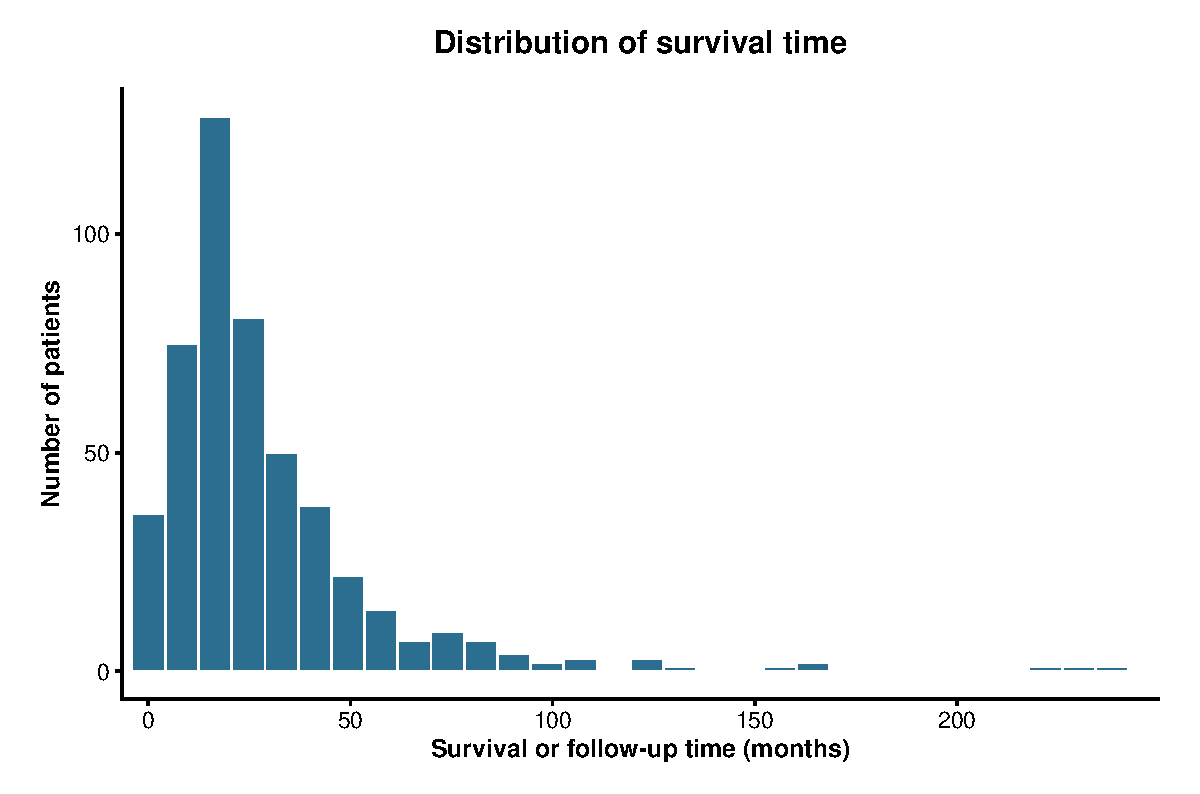
\includegraphics[width=0.92\textwidth]{distribuzione_tempo_sopravvivenza.pdf}
    \caption{Distribution of survival or follow-up time.}
    \label{fig:distribuzione_tempo}
\end{figure}

Observed time has a median of 21.4 months and an interquartile range of 13.7 to 36.1 months; the mean is 29.1 months. The distribution is strongly right-skewed: most patients have relatively short observed times, while a small number are followed for much longer periods, up to 238.3 months.

\subsubsection{Age at diagnosis}

The distribution of patients' age at diagnosis is shown in Figure~\ref{fig:distribuzione_eta}.

\begin{figure}[H]
    \centering
    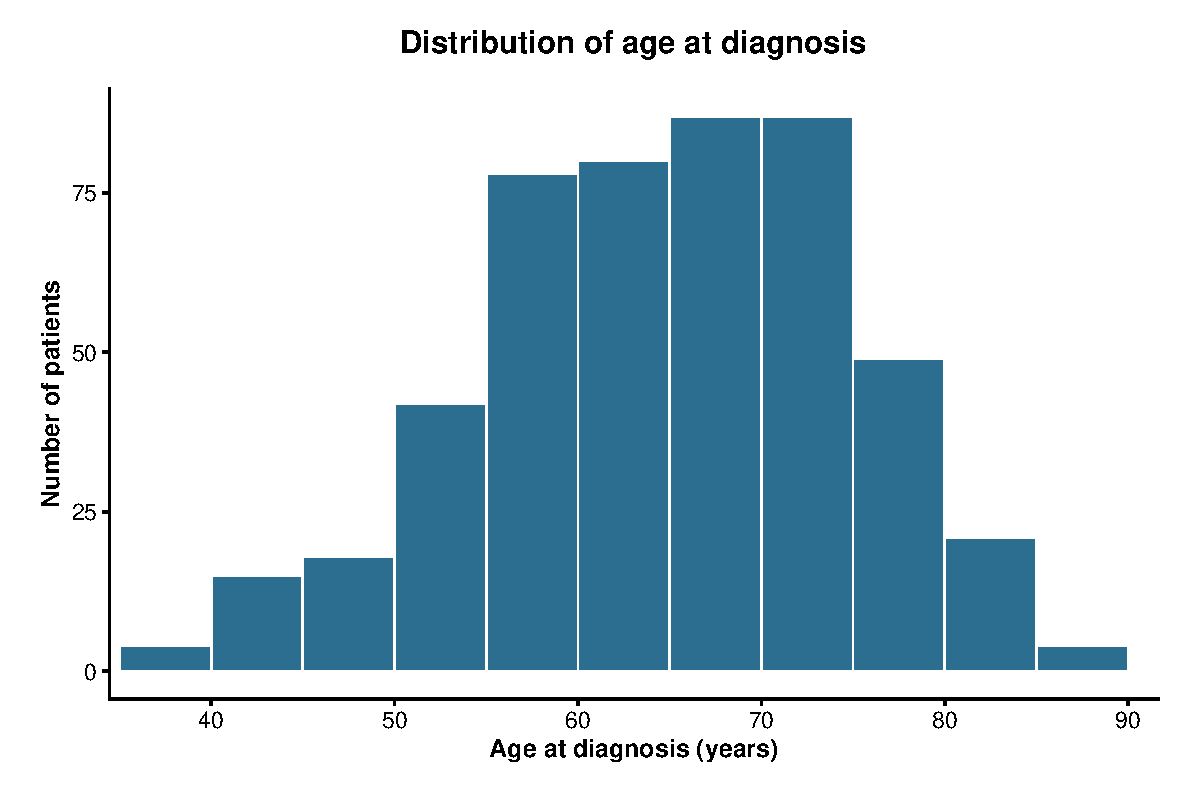
\includegraphics[width=0.92\textwidth]{distribuzione_eta.pdf}
    \caption{Distribution of age at diagnosis.}
    \label{fig:distribuzione_eta}
\end{figure}

Age is mainly concentrated between approximately 55 and 80 years, with few very young or particularly old patients. The distribution shows no anomalies that would prevent age from being used as a quantitative covariate in the Cox model.

\subsubsection{Categorical variables}

Sex, pathological stage and histological subtype distributions are shown separately in Figures~\ref{fig:distribuzione_sesso}, \ref{fig:distribuzione_stadio} and \ref{fig:distribuzione_istologia}.

\begin{figure}[H]
    \centering
    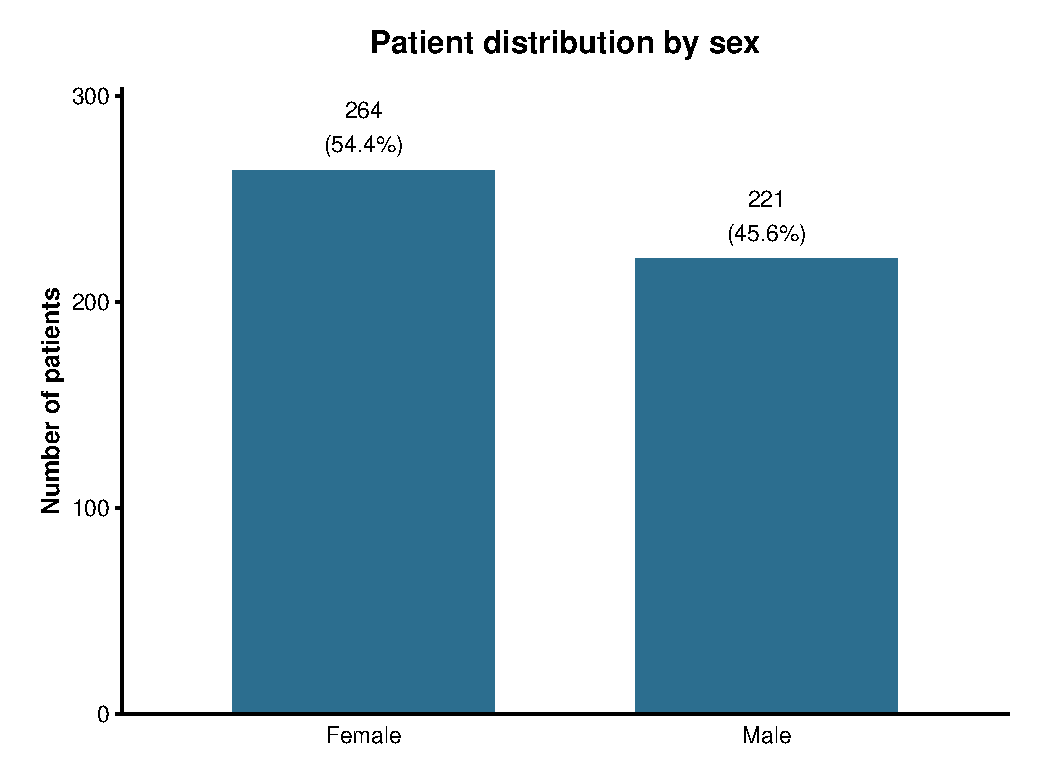
\includegraphics[width=0.78\textwidth]{distribuzione_sesso.pdf}
    \caption{Distribution of patients by sex.}
    \label{fig:distribuzione_sesso}
\end{figure}

There are 264 women (54.4\% of the sample) and 221 men (45.6\%).

\begin{figure}[H]
    \centering
    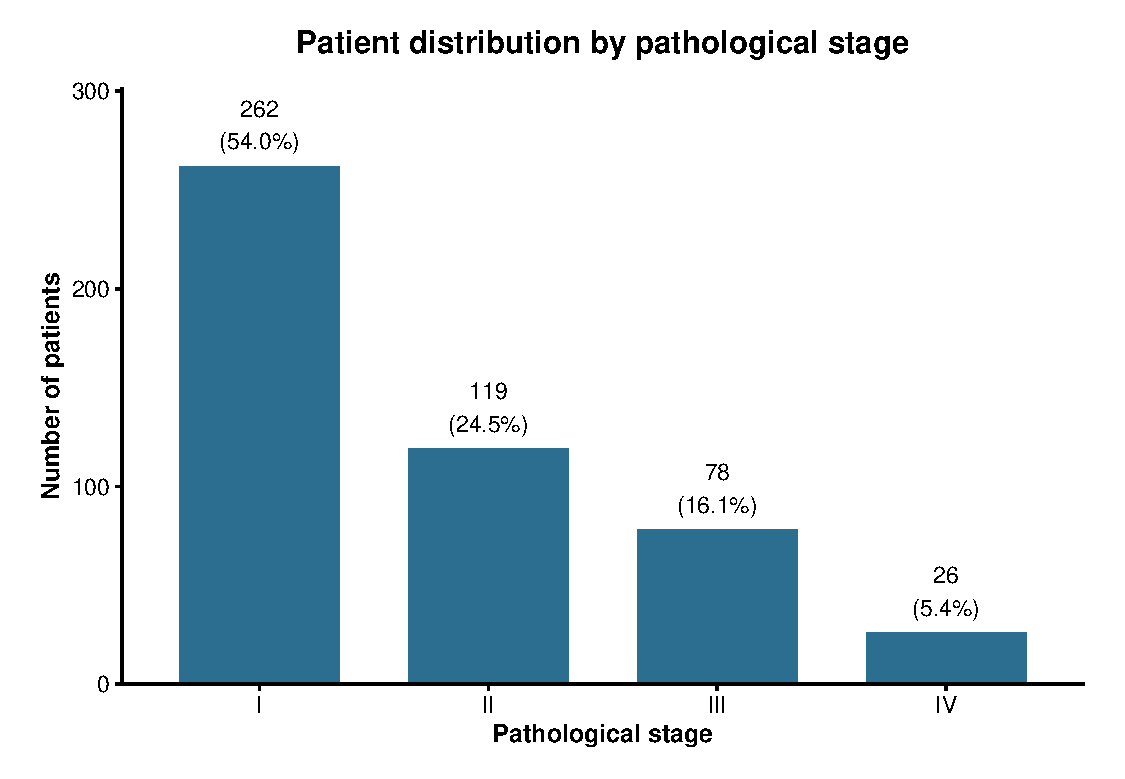
\includegraphics[width=0.82\textwidth]{distribuzione_stadio.pdf}
    \caption{Distribution of patients by pathological stage.}
    \label{fig:distribuzione_stadio}
\end{figure}

The distribution is skewed toward earlier stages: more than half of patients have stage I disease, while stage IV accounts for only 5.4\% of the sample. Estimates for stage IV therefore require greater caution.

\begin{figure}[H]
    \centering
    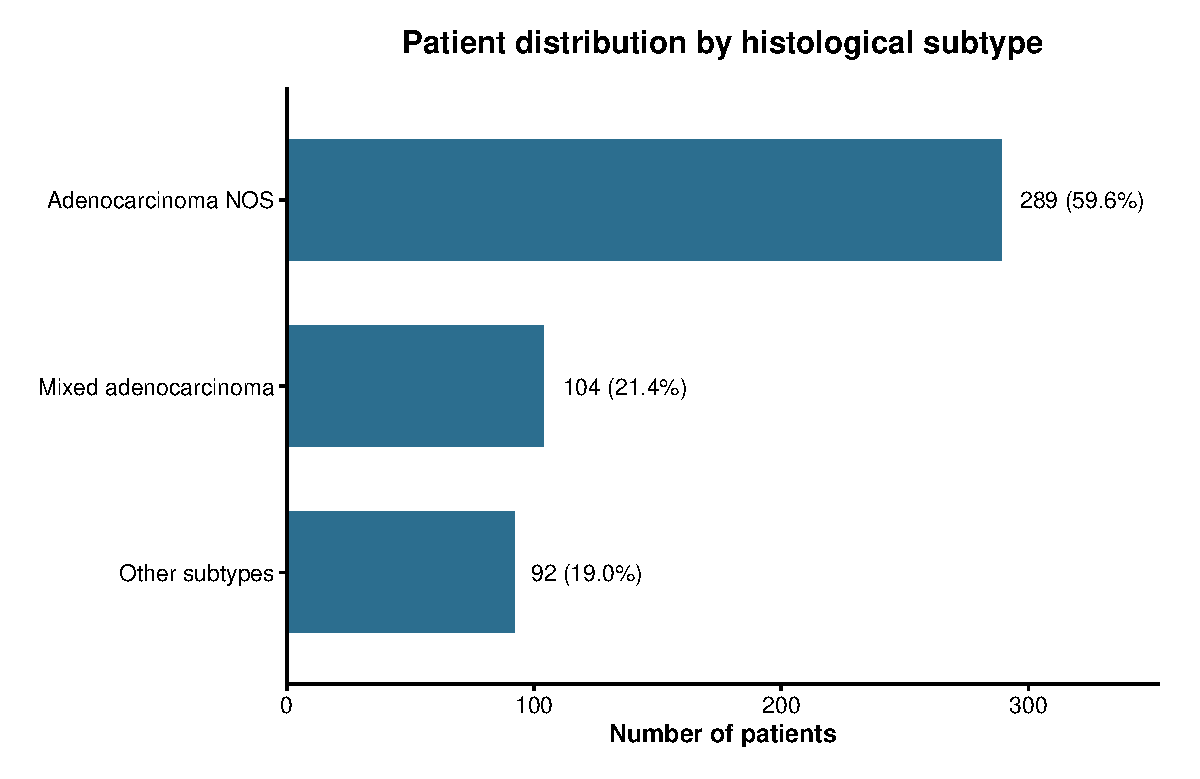
\includegraphics[width=0.88\textwidth]{distribuzione_istologia.pdf}
    \caption{Distribution of patients by histological subtype.}
    \label{fig:distribuzione_istologia}
\end{figure}

Adenocarcinoma NOS is the predominant category, accounting for approximately 60\% of the sample. The Other subtypes category is smaller and combines different histological forms, making it internally heterogeneous.

\subsubsection{Tumor-hypoxia indicators}

The dataset contains three tumor-hypoxia scores: Buffa Hypoxia Score, Ragnum Hypoxia Score and Winter Hypoxia Score. Each summarizes expression of a different gene signature responding to oxygen deprivation. These values are therefore not direct measurements of tissue oxygenation but relative molecular indices: a higher score indicates a tumor expression profile more consistent with a hypoxic response. Because the signatures use different gene sets and measurement scales, their absolute values should not be compared directly. Their respective distributions are shown in Figure~\ref{fig:distribuzione_hypoxia}.

\begin{figure}[H]
    \centering
    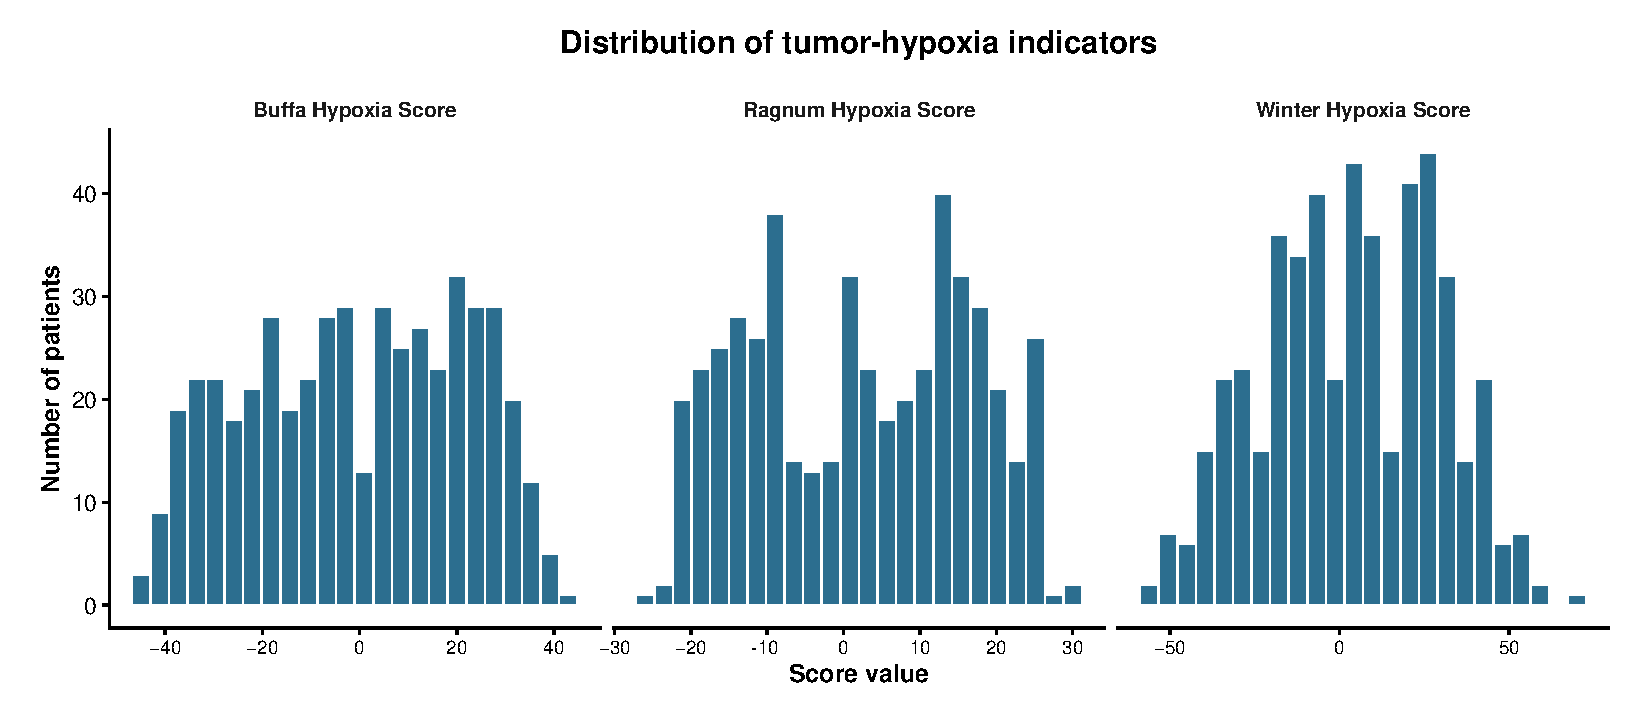
\includegraphics[width=\textwidth]{distribuzione_hypoxia_scores.pdf}
    \caption{Distribution of molecular tumor-hypoxia indicators.}
    \label{fig:distribuzione_hypoxia}
\end{figure}

All three scores take both negative and positive values and have fairly regular distributions without extreme tails requiring preliminary transformations. They are therefore initially treated as continuous quantitative variables in the models. Although measured on different scales, their linear associations can be compared using Pearson's correlation coefficient.

\subsection{Correlations}

The linear relationships among the three hypoxia indicators were assessed using Pearson's correlation coefficient. The matrix is shown in Figure~\ref{fig:correlazione_hypoxia}.

\begin{figure}[H]
    \centering
    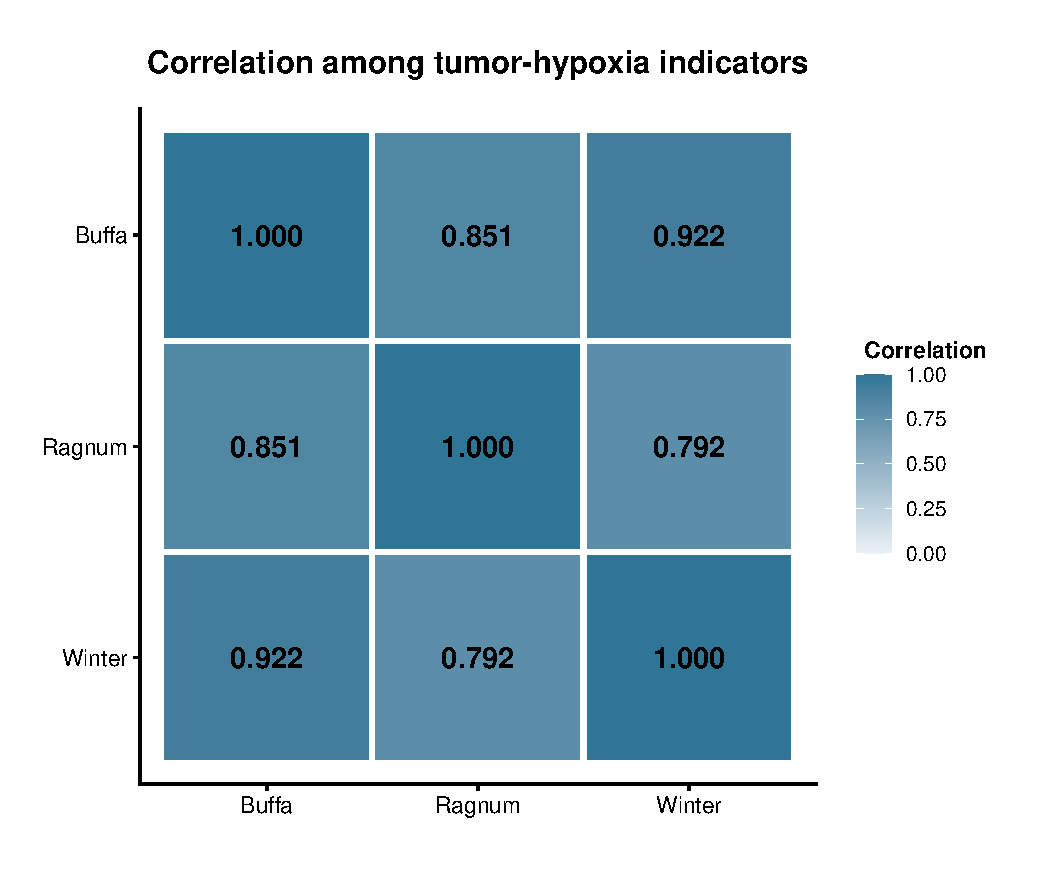
\includegraphics[width=0.76\textwidth]{correlazione_hypoxia_scores.pdf}
    \caption{Correlation matrix of tumor-hypoxia indicators.}
    \label{fig:correlazione_hypoxia}
\end{figure}

Correlations are high: the Buffa--Ragnum correlation is 0.851, Buffa--Winter is 0.922 and Ragnum--Winter is 0.792.

\begin{table}[H]
    \centering
    \caption{Correlations among tumor-hypoxia indicators.}
    \label{tab:correlazioni_hypoxia}
    \renewcommand{\arraystretch}{1.2}
    \begin{tabular}{l l c}
        \toprule
        \textbf{Indicator 1} & \textbf{Indicator 2} & \textbf{Correlation} \\
        \midrule
        Buffa  & Ragnum & 0,851 \\
        Buffa  & Winter & 0,922 \\
        Ragnum & Winter & 0,792 \\
        \bottomrule
    \end{tabular}
\end{table}

The strong association among the three scores suggests that they describe substantially overlapping components of the same biological phenomenon. Including them simultaneously in the model could therefore introduce collinearity and make estimates unstable. To keep the model parsimonious and interpretable, one indicator was selected: Buffa Hypoxia Score was used as the primary signature. Ragnum and Winter were used to examine the consistency of the molecular phenomenon, but were not entered into the model together. This is an operational choice, not evidence that the Buffa score is formally superior to the other two indicators.

% ================================================================
% 4. ANALISI DI SOPRAVVIVENZA
% ================================================================

\section{Survival analysis}

The survival function was estimated using the Kaplan--Meier method. Time was defined as the interval, in months, between diagnosis and death or, for patients without an observed event, between diagnosis and the last available contact. Patients alive at the end of follow-up were therefore treated as censored observations.

\subsection{Overall Kaplan--Meier curve}

The overall curve describes how survival probability changes in the study population. As shown in Figure~\ref{fig:km_complessiva}, estimated survival probability decreases progressively during follow-up, with a more pronounced decline in the early years and a subsequent tail with fewer patients remaining at risk.

\begin{figure}[H]
    \centering
    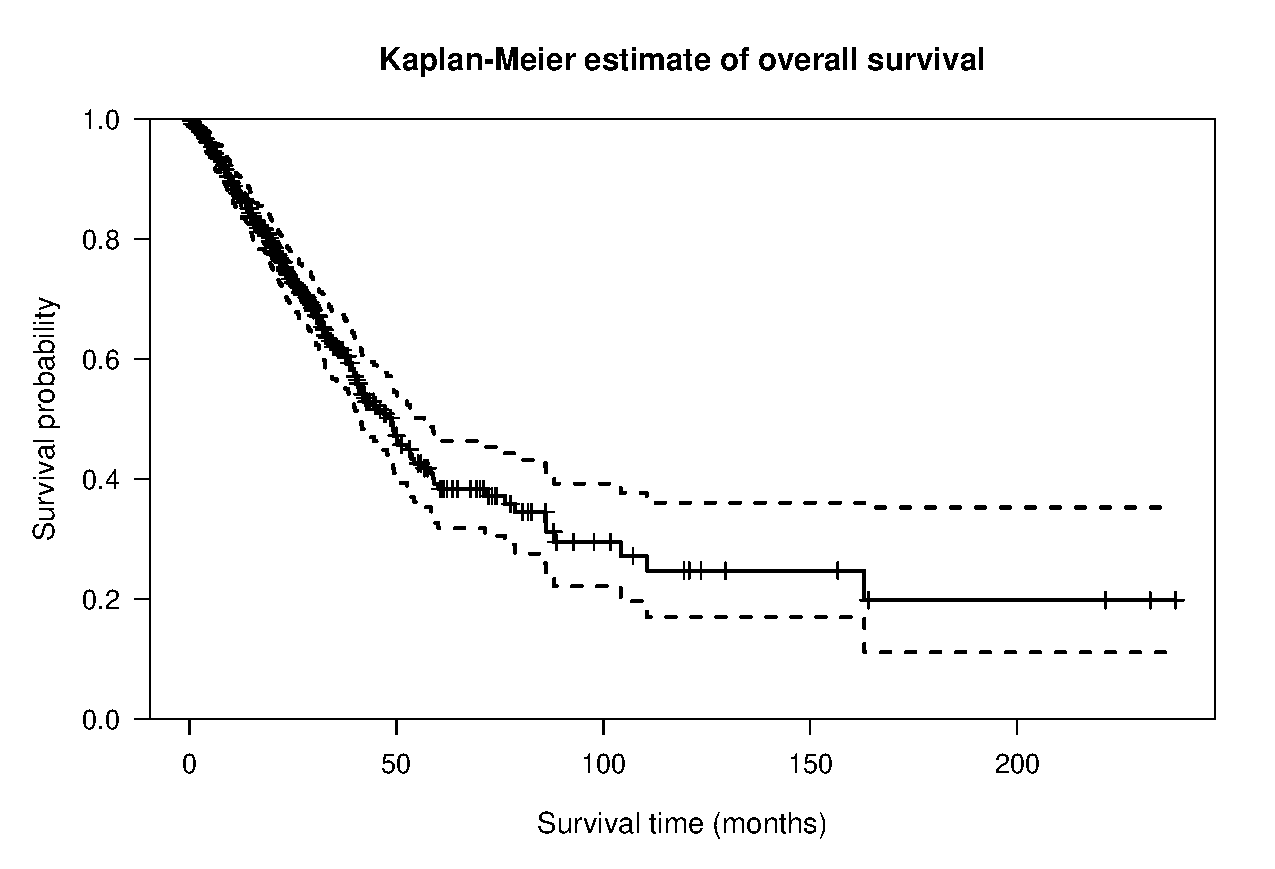
\includegraphics[width=0.92\textwidth]{km_complessiva.pdf}
    \caption{Overall Kaplan--Meier curve with a 95\% confidence interval.}
    \label{fig:km_complessiva}
\end{figure}

Estimated median survival is 49.1 months, with a 95\% confidence interval of 41.4 to 56.7 months. Estimated survival probabilities are 87.5\% at 12 months, 61.5\% at 36 months and 39.2\% at 60 months.

\subsection{Kaplan--Meier curves by pathological stage}

To assess the association between disease extent and survival, separate curves were estimated for the four pathological stages, as shown in Figure~\ref{fig:km_stadio}.

\begin{figure}[H]
    \centering
    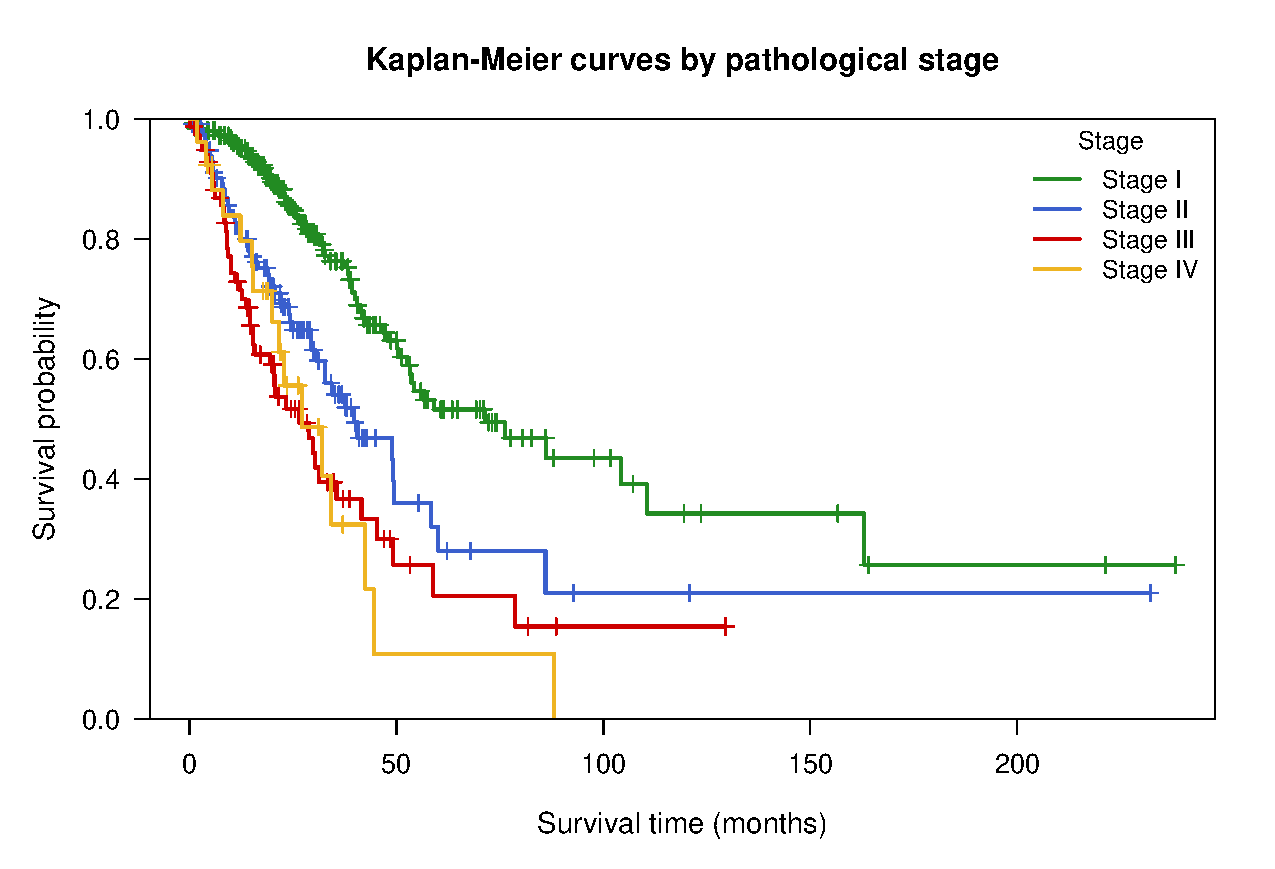
\includegraphics[width=0.92\textwidth]{km_stadio.pdf}
    \caption{Kaplan--Meier curves by pathological stage.}
    \label{fig:km_stadio}
\end{figure}

The stage I curve generally remains above the other curves, indicating a more favorable prognosis. Stages II, III and IV show progressively lower survival probabilities, with overall worse outcomes in the more advanced stages.

The log-rank test indicates a statistically significant difference among the four groups' survival curves:

\[
p < 0{,}001.
\]

Pathological stage is therefore strongly associated with overall survival in the unadjusted analysis. However, this comparison does not account for the patients' other clinical and molecular characteristics, which will subsequently be considered in the Cox model.

% ================================================================
% 4.2 MODELLO DI COX MULTIVARIATO E STRATIFICATO
% ================================================================

\subsection{Modello di Cox multivariato e stratificato}

Per valutare simultaneamente l'associazione tra le caratteristiche cliniche e molecolari dei pazienti e il rischio di morte è stato inizialmente stimato un modello di Cox multivariato a rischi proporzionali. Il modello comprende l'età alla diagnosi, il sesso, lo stadio patologico, il sottotipo istologico e il Buffa Hypoxia Score.

L'età è stata espressa in unità di dieci anni e il Buffa Hypoxia Score in unità di dieci punti, così da rendere più immediata l'interpretazione dei rispettivi hazard ratio. Le categorie di riferimento sono il sesso femminile, lo stadio I e l'adenocarcinoma NOS.

Il modello iniziale può essere espresso come:

\begin{equation}
\begin{split}
h(t \mid X)=h_0(t)\exp\{&
\beta_1 \mathrm{Et\grave{a}}_{10}
+\beta_2 \mathrm{Sesso}
+\beta_3 \mathrm{Stadio} \\
&+\beta_4 \mathrm{Istologia}
+\beta_5 \mathrm{Buffa}_{10}\}.
\end{split}
\label{eq:cox_standard}
\end{equation}

I risultati del modello multivariato standard sono riportati nella Tabella~\ref{tab:cox_standard}.

\begin{table}[H]
\centering
\caption{Modello di Cox multivariato standard.}
\label{tab:cox_standard}
\renewcommand{\arraystretch}{1.15}
\small
\begin{tabular}{l c c c}
\toprule
\textbf{Covariata}
& \textbf{HR}
& \textbf{IC 95\%}
& \textbf{$p$-value} \\
\midrule
Età, per 10 anni
& 1,236
& 1,052--1,452
& 0,010 \\

Maschio vs Femmina
& 1,013
& 0,750--1,367
& 0,933 \\

Stadio II vs I
& 1,931
& 1,334--2,795
& $<0,001$ \\

Stadio III vs I
& 2,888
& 1,960--4,255
& $<0,001$ \\

Stadio IV vs I
& 3,821
& 2,170--6,729
& $<0,001$ \\

Adenocarcinoma misto vs NOS
& 0,748
& 0,504--1,111
& 0,150 \\

Altri sottotipi vs NOS
& 0,477
& 0,282--0,807
& 0,006 \\

Buffa score, per 10 punti
& 1,117
& 1,036--1,206
& 0,004 \\
\bottomrule
\end{tabular}
\end{table}

Il modello risulta globalmente significativo secondo il likelihood ratio test ($p<0,001$).

A parità delle altre covariate, un incremento di dieci anni nell'età è associato a un aumento del rischio di morte pari a circa il 23,6\%. Il sesso non mostra invece un'associazione statisticamente significativa con l'evento.

Lo stadio patologico risulta fortemente associato alla prognosi. Rispetto allo stadio I, l'hazard è circa 1,9 volte maggiore nello stadio II, 2,9 volte maggiore nello stadio III e 3,8 volte maggiore nello stadio IV.

Per quanto riguarda l'istologia, l'adenocarcinoma misto non differisce significativamente dalla categoria NOS. La categoria degli altri sottotipi presenta invece un hazard inferiore, pari a 0,477. Infine, un aumento di dieci punti del Buffa Hypoxia Score è associato a un incremento dell'11,7\% del rischio di morte.

\subsubsection{Verifica dell'ipotesi di rischi proporzionali}

L'assunzione di proporzionalità degli hazard è stata verificata mediante il test basato sui residui di Schoenfeld. I risultati relativi al modello standard sono riportati nella Tabella~\ref{tab:schoenfeld_standard}.

\begin{table}[H]
\centering
\caption{Test di Schoenfeld per il modello di Cox multivariato standard.}
\label{tab:schoenfeld_standard}
\renewcommand{\arraystretch}{1.15}
\begin{tabular}{l c c c}
\toprule
\textbf{Covariata}
& \textbf{Chi-quadro}
& \textbf{gdl}
& \textbf{$p$-value} \\
\midrule
Età
& 1,611
& 1
& 0,204 \\

Sesso
& 5,021
& 1
& 0,025 \\

Stadio patologico
& 10,313
& 3
& 0,016 \\

Sottotipo istologico
& 0,445
& 2
& 0,801 \\

Buffa Hypoxia Score
& 1,461
& 1
& 0,227 \\

\textbf{Globale}
& \textbf{18,719}
& \textbf{8}
& \textbf{0,016} \\
\bottomrule
\end{tabular}
\end{table}

Il test non evidenzia violazioni per l'età, il sottotipo istologico e il Buffa Hypoxia Score. Al contrario, il sesso e lo stadio patologico presentano valori di $p$ inferiori a 0,05. Anche il test globale risulta significativo, indicando che il modello standard non soddisfa pienamente l'ipotesi di rischi proporzionali. Per il sesso, la non significatività dell'hazard ratio medio non esclude una possibile variazione dell'effetto nel tempo.

In Figura~\ref{fig:schoenfeld_sesso_stadio} vengono riportati esclusivamente i residui di Schoenfeld relativi al sesso e allo stadio patologico, cioè le covariate per le quali il test ha evidenziato una possibile variazione dell'effetto nel tempo.

\begin{figure}[H]
\centering
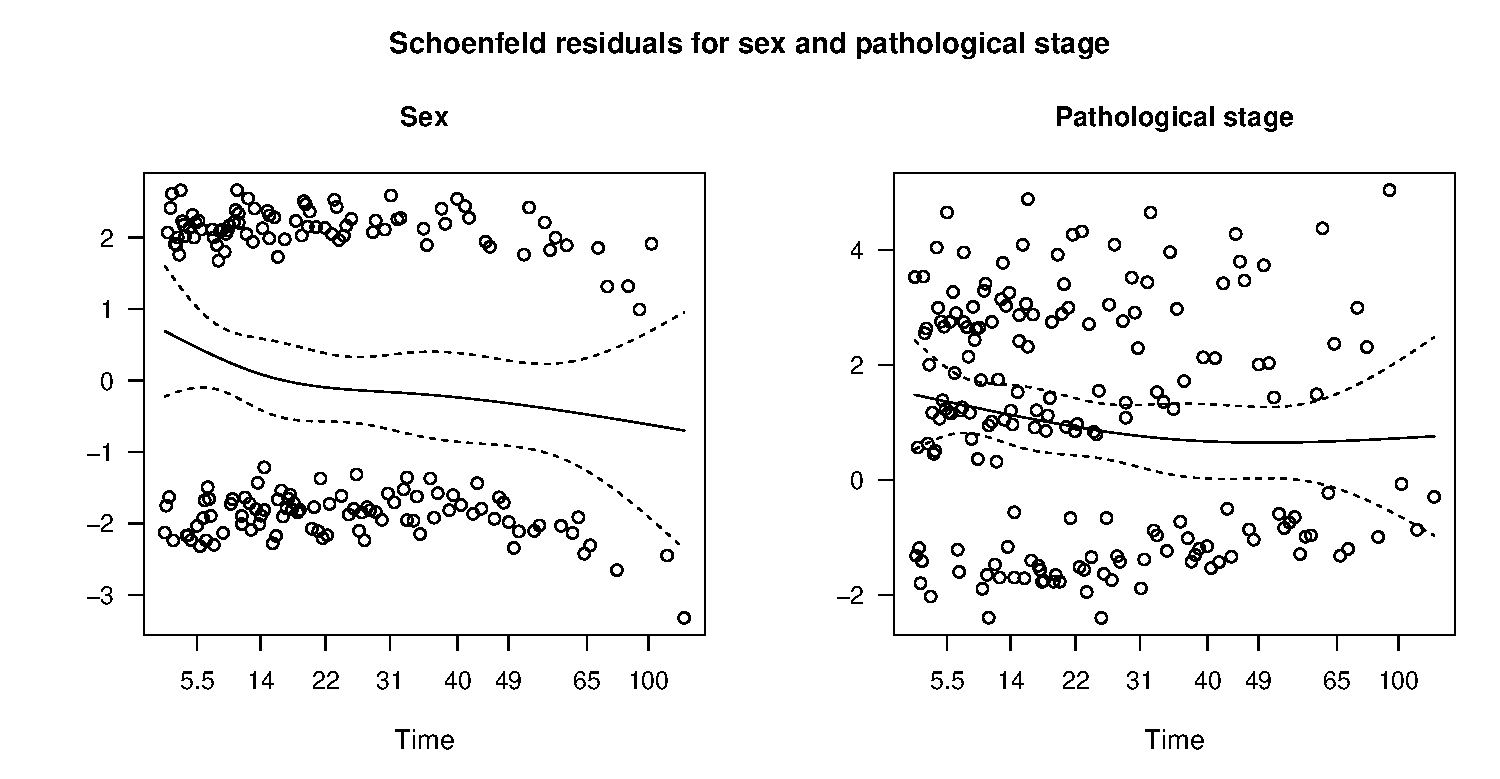
\includegraphics[width=0.95\textwidth]{schoenfeld_sesso_stadio.pdf}
\caption{Residui di Schoenfeld per sesso e stadio patologico.}
\label{fig:schoenfeld_sesso_stadio}
\end{figure}

I grafici confermano che l'effetto del sesso e dello stadio patologico non rimane costante durante il follow-up. In particolare, le curve smussate dei coefficienti stimati mostrano un andamento non perfettamente orizzontale nel tempo, coerente con i risultati significativi del test di Schoenfeld.

Poiché l'ipotesi di rischi proporzionali non risulta soddisfatta per queste due covariate, è stato successivamente stimato un modello di Cox stratificato per sesso e stadio patologico. In questo modo, ciascuna combinazione delle due variabili può avere una propria funzione di rischio di base, senza imporre un effetto costante nel tempo.

\subsubsection{Modello di Cox stratificato}

Per gestire la violazione dell'ipotesi di proporzionalità è stato stimato un modello di Cox stratificato congiuntamente per stadio patologico e sesso. La stratificazione consente a ciascuna combinazione di stadio e sesso di possedere una propria funzione di rischio di base, senza imporre che gli effetti di queste due variabili rimangano costanti durante il follow-up.

Il modello finale è:

\begin{equation}
h_s(t \mid X)
=
h_{0s}(t)
\exp\{
\beta_1 \mathrm{Et\grave{a}}_{10}
+\beta_2 \mathrm{Istologia}
+\beta_3 \mathrm{Buffa}_{10}
\},
\label{eq:cox_stratificato}
\end{equation}

dove $s$ identifica lo strato definito dalla combinazione tra stadio patologico e sesso. La stratificazione consente quindi funzioni di rischio di base differenti per le combinazioni osservate delle due variabili, fino a un massimo teorico di otto strati. Il costo di questa scelta è che il modello non restituisce un unico hazard ratio per sesso e stadio patologico, poiché i loro effetti vengono assorbiti nelle funzioni di rischio di base specifiche di strato.

I risultati del modello stratificato finale sono riportati nella Tabella~\ref{tab:cox_stratificato}.

\begin{table}[H]
\centering
\caption{Modello di Cox stratificato per stadio patologico e sesso.}
\label{tab:cox_stratificato}
\renewcommand{\arraystretch}{1.15}
\small
\begin{tabular}{l c c c}
\toprule
\textbf{Covariata}
& \textbf{HR}
& \textbf{IC 95\%}
& \textbf{$p$-value} \\
\midrule
Età, per 10 anni
& 1,241
& 1,055--1,460
& 0,009 \\

Adenocarcinoma misto vs NOS
& 0,769
& 0,516--1,144
& 0,195 \\

Altri sottotipi vs NOS
& 0,473
& 0,275--0,812
& 0,007 \\

Buffa score, per 10 punti
& 1,107
& 1,025--1,196
& 0,010 \\
\bottomrule
\end{tabular}
\end{table}

Il modello stratificato risulta globalmente significativo secondo il likelihood ratio test ($p<0,001$).

Anche dopo aver consentito a stadio e sesso di possedere rischi di base differenti, l'età e il Buffa Hypoxia Score rimangono significativamente associati alla sopravvivenza. Un aumento di dieci anni nell'età determina un incremento dell'hazard pari a circa il 24,1\%, mentre un aumento di dieci punti del Buffa score è associato a un incremento del rischio pari al 10,7\%.

Gli altri sottotipi istologici continuano a mostrare un hazard inferiore rispetto all'adenocarcinoma NOS, mentre l'adenocarcinoma misto non presenta una differenza statisticamente significativa.

\subsubsection{Verifica del modello stratificato}

Il test di Schoenfeld è stato ripetuto sulle covariate stimate nel modello stratificato. I risultati sono riportati nella Tabella~\ref{tab:schoenfeld_stratificato}.

\begin{table}[H]
\centering
\caption{Test di Schoenfeld per il modello di Cox stratificato.}
\label{tab:schoenfeld_stratificato}
\renewcommand{\arraystretch}{1.15}
\begin{tabular}{l c c c}
\toprule
\textbf{Covariata}
& \textbf{Chi-quadro}
& \textbf{gdl}
& \textbf{$p$-value} \\
\midrule
Età
& 2,796
& 1
& 0,095 \\

Sottotipo istologico
& 0,167
& 2
& 0,920 \\

Buffa Hypoxia Score
& 0,191
& 1
& 0,662 \\

\textbf{Globale}
& \textbf{3,613}
& \textbf{4}
& \textbf{0,461} \\
\bottomrule
\end{tabular}
\end{table}

Tutti i valori di $p$ risultano superiori a 0,05 e il test globale non è significativo. Non emerge quindi evidenza di una violazione residua dell'ipotesi di rischi proporzionali. Per questo motivo non vengono riportati ulteriori grafici dei residui di Schoenfeld per il modello stratificato.

Il modello stratificato viene pertanto considerato il modello finale, poiché consente di gestire la non proporzionalità di sesso e stadio mantenendo nel modello le associazioni relative all'età, al sottotipo istologico e all'ipossia tumorale. Tale scelta comporta tuttavia la rinuncia alla stima di un unico hazard ratio per le due variabili utilizzate nella stratificazione.

\subsection{Diagnostica del modello definitivo}

Per valutare l'adeguatezza della forma funzionale delle covariate continue incluse nel modello stratificato finale sono stati analizzati i residui di Martingala rispetto all'età e al Buffa Hypoxia Score.

\begin{figure}[H]
\centering
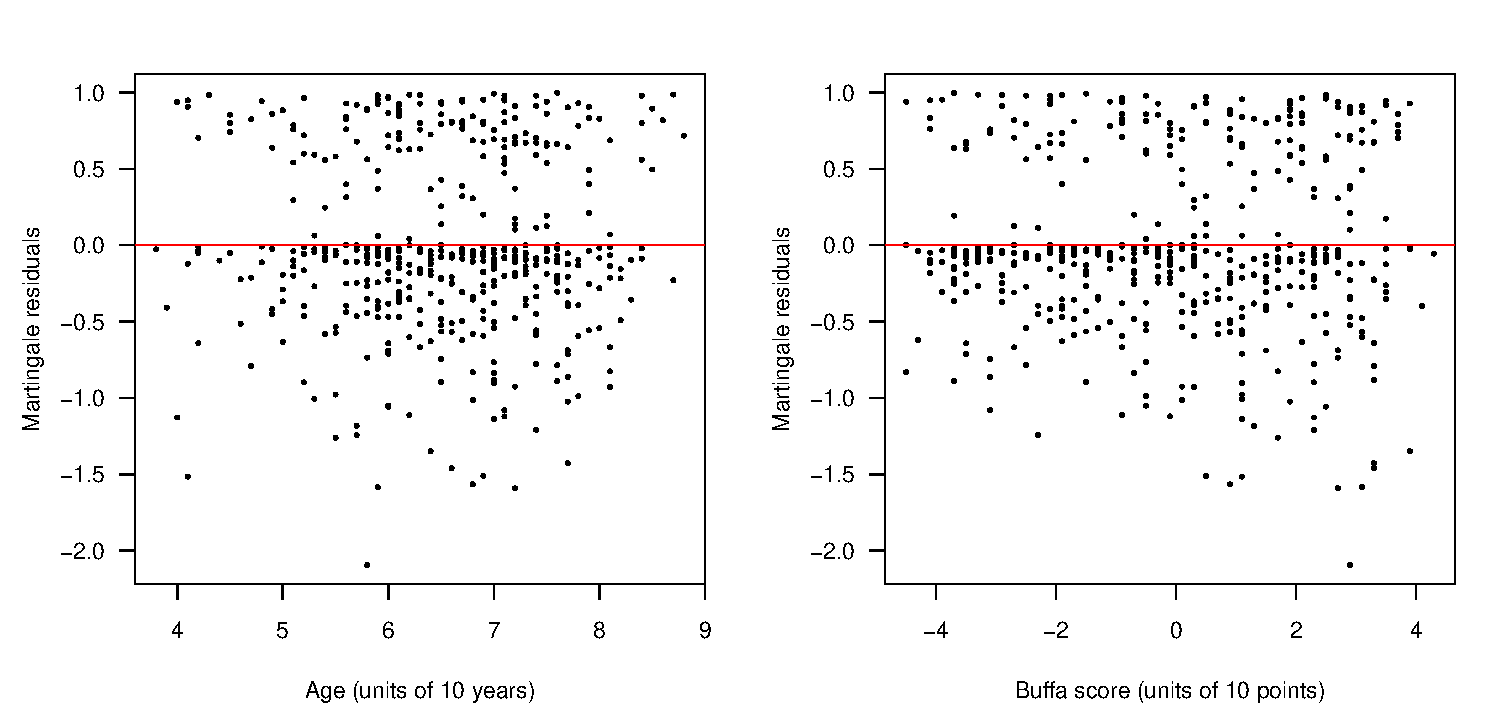
\includegraphics[width=0.95\textwidth]{martingala_eta_buffa.pdf}
\caption{Residui di Martingala rispetto all'età e al Buffa Hypoxia Score.}
\label{fig:martingala_eta_buffa}
\end{figure}

La linea rossa orizzontale rappresenta il valore di riferimento pari a zero. In entrambi i grafici i residui risultano dispersi al di sopra e al di sotto di tale linea, senza evidenziare pattern sistematici particolarmente marcati rispetto all'età o al Buffa Hypoxia Score. L'analisi grafica non suggerisce quindi deviazioni evidenti dalla forma funzionale lineare adottata nel modello.

\subsection{Profili prognostici clinico-molecolari}

Per illustrare l'effetto congiunto dell'età e dell'ipossia tumorale sono stati definiti tre profili ipotetici. Il profilo favorevole corrisponde a una paziente di 55 anni con Buffa Hypoxia Score pari a $-20$, quello intermedio a una paziente di 65 anni con score pari a 0 e quello sfavorevole a una paziente di 75 anni con score pari a 20. In tutti e tre i profili sono stati mantenuti costanti il sesso femminile, lo stadio I e il sottotipo istologico Adenocarcinoma NOS.

\begin{figure}[H]
\centering
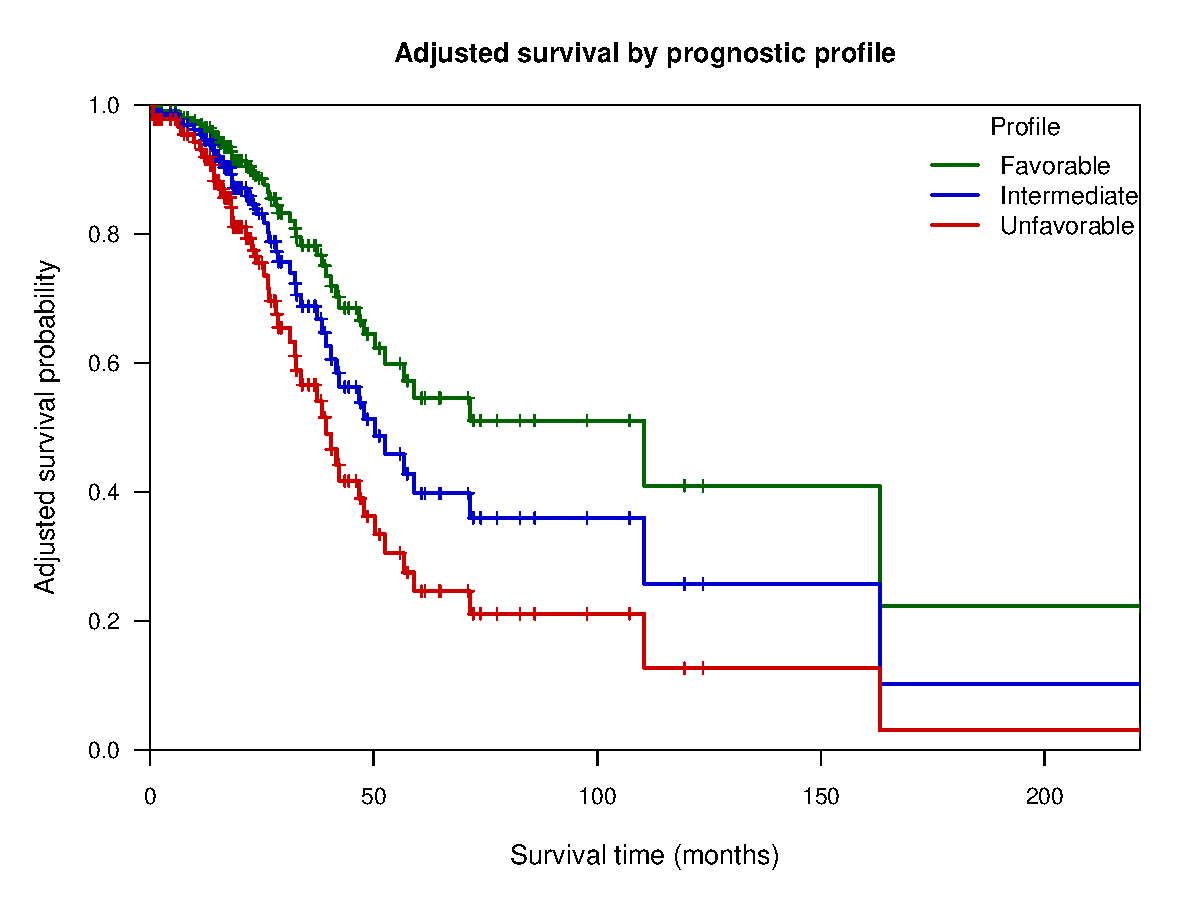
\includegraphics[width=0.95\textwidth]{curve_profili_prognostici.pdf}
\caption{Curve di sopravvivenza stimata per i tre profili prognostici clinico-molecolari.}
\label{fig:profili_prognostici}
\end{figure}

Le curve mostrano un gradiente prognostico netto. A 60 mesi, la sopravvivenza stimata è pari a 0,546 per il profilo favorevole, 0,398 per quello intermedio e 0,246 per quello sfavorevole. La separazione riflette l'effetto combinato di età e Buffa Hypoxia Score secondo il modello stimato.

\section{Limiti dello studio}

I risultati devono essere interpretati considerando alcuni limiti. In primo luogo, l'analisi utilizza dati osservazionali e retrospettivi, per cui le associazioni stimate non possono essere interpretate in senso causale. Inoltre, è stata adottata un'analisi per casi completi: la quota di osservazioni escluse è contenuta, ma la validità delle stime richiede che i dati mancanti non introducano differenze sistematiche rilevanti tra pazienti inclusi ed esclusi.

La numerosità dello stadio IV è ridotta e la stratificazione congiunta per stadio e sesso suddivide ulteriormente il campione in combinazioni meno numerose. Le stime relative agli strati meno rappresentati devono quindi essere interpretate con cautela. Infine, la categoria ``Altri sottotipi'' riunisce forme istologiche differenti e può nascondere una certa eterogeneità interna.

\section{Conclusioni}

L'analisi evidenzia che età alla diagnosi, Buffa Hypoxia Score e sottotipo istologico sono associati alla sopravvivenza dei pazienti con adenocarcinoma polmonare. In particolare, un aumento di dieci anni nell'età corrisponde a un incremento dell'hazard di circa il 24\%, mentre un aumento di dieci punti del Buffa score è associato a un incremento di circa l'11\%.

Lo stadio patologico risulta fortemente associato alla prognosi nel modello standard. Poiché sesso e stadio non soddisfano l'ipotesi di rischi proporzionali, è stato adottato un modello stratificato, che elimina l'evidenza di violazioni residue e mantiene le associazioni relative alle altre covariate.

Nel complesso, i risultati indicano che l'integrazione tra caratteristiche cliniche e ipossia tumorale consente di distinguere livelli prognostici differenti, pur con i limiti legati alla natura osservazionale dei dati e alla ridotta numerosità di alcuni sottogruppi.

\section{Fonti}

I dati utilizzati nell'analisi provengono dallo studio
\textit{Lung Adenocarcinoma (TCGA, PanCancer Atlas)}, disponibile su cBioPortal for Cancer Genomics:

\begin{center}
\href{https://www.cbioportal.org/study/summary?id=luad_tcga_pan_can_atlas_2018}
{\texttt{https://www.cbioportal.org/study/summary?id=luad\_tcga\_pan\_can\_atlas\_2018}}
\end{center}

\end{document}